% Circuits were set up in LTspice.

\documentclass[11pt]{article}

\usepackage{graphicx}
\usepackage[top=25mm, bottom=25mm, left=25mm, right=25mm, a4paper]{geometry}
\usepackage{amsmath}
\usepackage{enumitem}
\usepackage{float}
\usepackage{fancyhdr}
\usepackage{booktabs}
\usepackage{tikz}
\usepackage{steinmetz}

\pagestyle{fancy}
\fancyhf{}
\fancyhead[R]{Baturay Kafkas - 2240357068 - Electrical \& Electronics Engineering}

\rfoot{\thepage}
\renewcommand{\headrulewidth}{0pt} 
\renewcommand{\footrulewidth}{0pt}
\sloppy

\begin{document}

\begin{center}
\large
\textbf{ELE226 Circuit Theory II Homework 1}
\end{center}

\section{Questions}

\begin{enumerate}[leftmargin=*,label=\textbf{\arabic*.}]

\item \textit{J. W. Nilsson and S. Riedel, Electric Circuits, 10th ed., Pearson, 2014, Problem 11.1, p. 418}
\item \textit{J. W. Nilsson and S. Riedel, Electric Circuits, 10th ed., Pearson, 2014, Example 11.1, p. 403}
\item \textit{J. W. Nilsson and S. Riedel, Electric Circuits, 10th ed., Pearson, 2014, Problem 11.39, p. 423}
\item \textit{J. W. Nilsson and S. Riedel, Electric Circuits, 10th ed., Pearson, 2014, Problem 11.50, p. 424}

\end{enumerate}

\section{Answers}

\begin{enumerate}[leftmargin=*,label=\textbf{\arabic*.}]

\item \textbf{a.} The b-phase voltage lags the a-phase voltage by $120^\circ$. The a-phase voltage lags the c-phase voltage by $120^\circ$. Therefore, it corresponds to a positive phase sequence (abc).

\textbf{b.} Convert $v_c$ into cosine form.
\[v_c=820\sin(\omega t-66^\circ)=820\cos(\omega t -156^\circ)\qquad [\sin(\theta)=\cos(\theta-90^\circ)]\]

The c-phase voltage lags the a-phase voltage by $120^\circ$. The a-phase voltage lags the b-phase voltage by $120^\circ$. Therefore, it corresponds to a negative phase sequence (acb).

\item \textbf{a.} The a-phase equivalent circuit is as follows.
\begin{figure}[H]
    \centering
    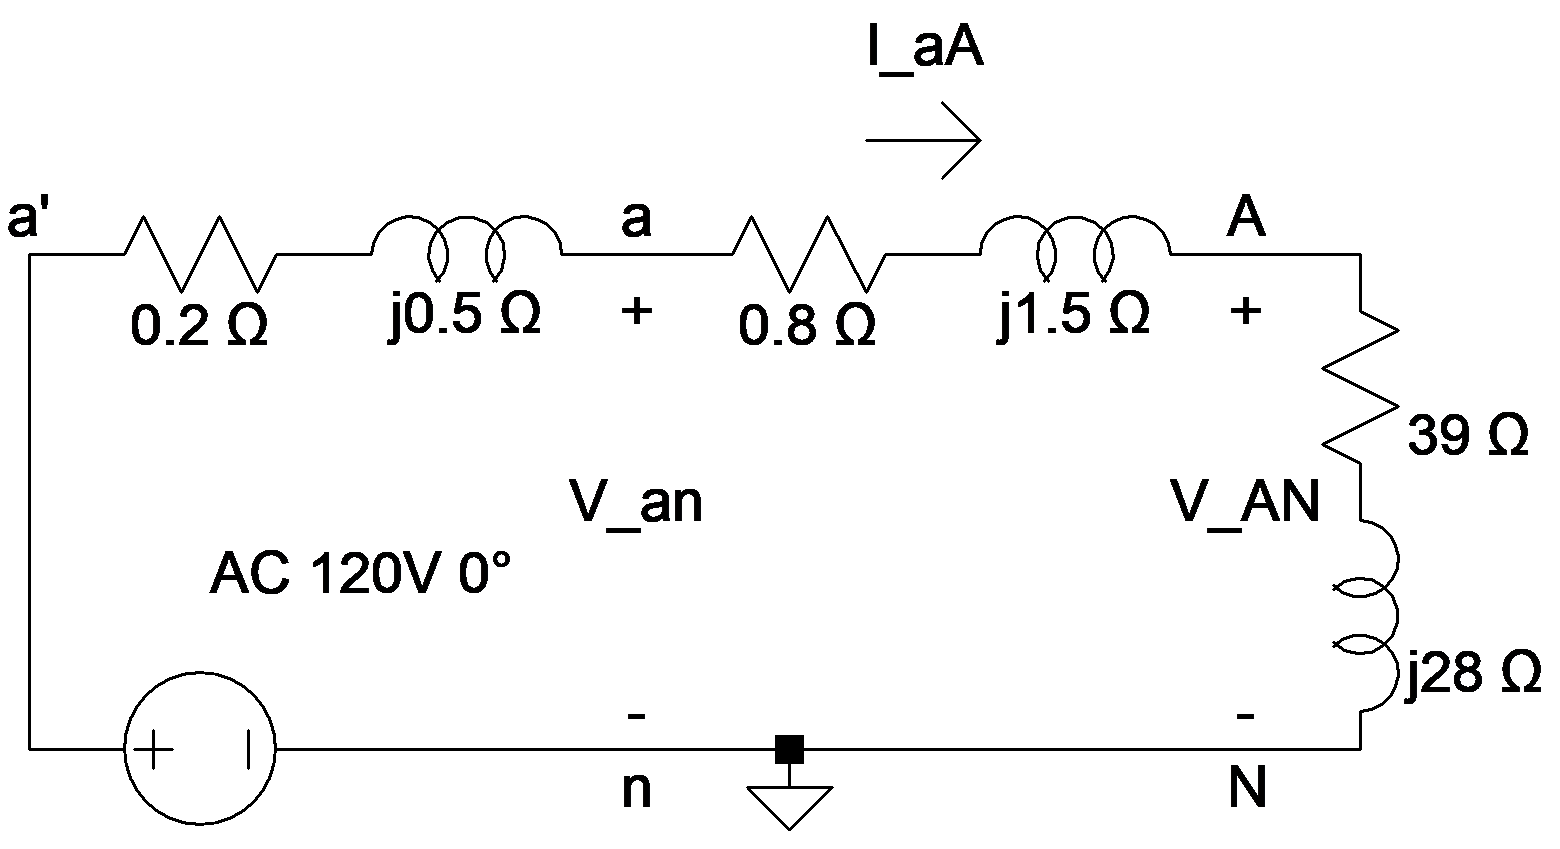
\includegraphics[width=0.6\linewidth]{image.png}
\end{figure}

\vspace{1em}

\textbf{b.} We first calculate $\mathbf{I}_{\text{aA}}$. By Ohm's law,
\begin{align*}\mathbf{I}_{\text{aA}}=\frac{120\,\phase{0^{\circ}}}{(0.2 + j0.5)+(0.8+j1.5)+(39+j28)}&=\frac{120\,\phase{0^{\circ}}}{(0.2+0.8+39)+j(0.5+1.5+28)}\\[1em]&=\frac{120\,\phase{0^{\circ}}}{40+j30}=2.4\,\phase{-36.87^{\circ}}\text{ A}.\end{align*}

Since the generator has a positive sequence, the rest become
\[\mathbf{I}_{\text{bB}}=2.4\,\phase{-156.87^{\circ}}\text{ A},\qquad \mathbf{I}_{\text{cC}}=2.4\,\phase{83.13^{\circ}}\text{ A}.\]

\newpage

\textbf{c.} Calculate the line voltages.
\[\mathbf{V}_{\text{AN}}=(39+j28)(2.4\,\phase{-36.87^{\circ}})=115.22\,\phase{-1.19^{\circ}}\text{ V}.\]

Similarly,
\[\mathbf{V}_{\text{BN}}=115.22\,\phase{-121.19^{\circ}}\text{ V},\qquad\mathbf{V}_{\text{CN}}=115.22\,\phase{118.81^{\circ}}\text{ V}.\]

\vspace{1em}

\textbf{d.} The line voltage $\mathbf{V}_{\text{AB}}$ can be calculate with the formula
\[\mathbf{V}_{\text{AB}}=\left(\sqrt3\phase{30^\circ}\right)\mathbf{V}_{\text{AN}}.\]

Therefore,
\[\mathbf{V}_{\text{AB}}=199.58\,\phase{28.81^\circ}\text{ V},\qquad\mathbf{V}_{\text{BC}}=199.58\,\phase{-91.19^\circ}\text{ V},\qquad\mathbf{V}_{\text{CA}}=199.58\,\phase{148.81^\circ}\text{ V}.\]

\vspace{1em}

\textbf{e.} We calculate the phase voltage by the following. By definition,
\[\mathbf{V}_{\text{an}}=120-(0.2+j0.5)(2.4\,\phase{-36.87^\circ})=120-1.29\,\phase{31.33^\circ}=118.90\,\phase{-0.32^\circ}\text{ V}\]

Similarly,
\[\mathbf{V}_{\text{bn}}=118.90\,\phase{-120.32^\circ}\text{ V},\qquad \mathbf{V}_{\text{cn}}=118.90\,\phase{119.68^\circ}\text{ V}.\]

\vspace{1em}

\textbf{f.} Like what we did in \textbf{(d)}, calculate the line voltages.
\[\mathbf{V}_{\text{ab}}=\left(\sqrt3\,\phase{30^\circ}\right)\mathbf{V}_{\text{an}}.\]

Therefore,
\[\mathbf{V}_{\text{ab}}=205.94\,\phase{29.68^\circ}\text{ V},\qquad\mathbf{V}_{\text{bc}}=205.94\,\phase{-90.32^\circ}\text{ V},\qquad\mathbf{V}_{\text{ca}}=205.94\,\phase{149.68^\circ}\text{ V}.\]

\vspace{1em}

\textbf{g.} The values for the negative phase sequence:
\[\mathbf{I}_{\text{aA}}=2.4\,\phase{-36.87^{\circ}}\text{ A},\qquad\mathbf{I}_{\text{bB}}=2.4\,\phase{83.13^{\circ}}\text{ A},\qquad \mathbf{I}_{\text{cC}}=2.4\,\phase{-156.87^{\circ}}\text{ A},\]
\[\mathbf{V}_{\text{AN}}=115.22\,\phase{-1.19^{\circ}}\text{ V},\qquad\mathbf{V}_{\text{BN}}=115.22\,\phase{118.81^{\circ}}\text{ V},\qquad\mathbf{V}_{\text{CN}}=115.22\,\phase{-121.19^{\circ}}\text{ V},\]
\[\mathbf{V}_{\text{AB}}=199.58\,\phase{-31.19^\circ}\text{ V},\qquad\mathbf{V}_{\text{BC}}=199.58\,\phase{88.81^\circ}\text{ V},\qquad\mathbf{V}_{\text{CA}}=199.58\,\phase{-151.19^\circ}\text{ V},\]
\[\mathbf{V}_{\text{an}}=118.90\,\phase{-0.32^\circ}\text{ V},\qquad\mathbf{V}_{\text{bn}}=118.90\,\phase{119.68^\circ}\text{ V},\qquad \mathbf{V}_{\text{cn}}=118.90\,\phase{-120.32^\circ}\text{ V},\]
\[\mathbf{V}_{\text{ab}}=205.94\,\phase{-30.32^\circ}\text{ V},\qquad\mathbf{V}_{\text{bc}}=205.94\,\phase{89.68^\circ}\text{ V},\qquad\mathbf{V}_{\text{ca}}=205.94\,\phase{-150.32^\circ}\text{ V}.\]

\vspace{1em}

\item \textbf{a.} The total power associated is $P=\sqrt3V_{L}I_{L}\cos(\phi)$.
\[P=\sqrt3V_{L}I_{L}\cos(\phi)\implies900\times10^3=\sqrt3\cdot2500\sqrt3\cdot I_L\cdot\cos(30^\circ)\implies I_L=200\:\text{A}\]
\[\arccos(0.6)=53.13^\circ\implies\mathbf{I}_L=200\,\phase{-53.13^\circ}\qquad[\text{lagging}]\]

The voltage across the impedance:
\[(1+j3)(200\,\phase{-53.13^\circ})=600+j200\text{ V}.\]

The voltage across the impedance and the load:
\[2500+600+j200=3100+j200\text{ V}.\]

The magnitude of the voltage across the sending end is then
\[\sqrt3\cdot|3100+j200|=5.38\text{ kV}.\]

\textbf{b.} The complex power associated with the capacitors:
\[S=-j\frac13(1125)\cdot10^3=-j375\:\text{kVAR}.\]

From the formula $S=\mathbf{V}\mathbf{I}$*, we find the current through the bank.
\[\mathbf{I}\text{*}=\frac{S}{\mathbf{V}}=\frac{-j375000}{2500}=-j150\text{ A}\implies\mathbf{I}=j150\text{ A}\]

The line current is $200\,\phase{-53.13^\circ}+j150=120-j10\text{ A}$. The phase voltage is
\[2500+(1+j3)(120-j10)=2650+j350\text{ V}.\]

The magnitude of the voltage across the sending end is then
\[\sqrt3|2650+j350|=4.63\text{ kV}.\]

\textbf{c.} The total average power delivered to the impedance is $P=3I^2R=3\cdot200^2\cdot1=120\text{ kW}$.
\[\text{\% efficiency}=\frac{900}{900+120}\cdot100=88.2\%\]

\textbf{d.} The total average power delivered to the impedance is $P=3I^2R=3\cdot120^2\cdot1=43.2\text{ kW}$.
\[\text{\% efficiency}=\frac{900}{900+43.2}\cdot100=95.4\%\]

\textbf{e.} The reactive power associated for one capacitor is $Q_C=\dfrac{V_\phi^2}{X_C}$. Therefore,
\[X_C=\frac{V_\phi^2}{Q_C}=\frac{2500^2}{\dfrac13\cdot 1125\cdot10^3}=16.67\:\Omega.\]

The capacitive reactance is defined as $\dfrac1{wC}$. From here,
\[C=\frac1{16.67\cdot120\pi}=159\:\mu\text{F}.\]

\vspace{1em}

\item \textbf{a.} Transforming the $\Delta$ into the wye form, we get
\[\mathbf{I}_\text{aA}=\frac{240\,\phase{0^\circ}}{\dfrac{40}{3}\,\phase{-30^\circ}}=18\,\phase{30^\circ}\text{ A},\qquad\mathbf{I}_\text{bB}=\frac{240\,\phase{120^\circ}}{\dfrac{40}{3}\,\phase{-30^\circ}}=18\,\phase{150^\circ}\text{ A},\]
\[\mathbf{I}_\text{cC}=\frac{240\,\phase{-120^\circ}}{\dfrac{40}{3}\,\phase{-30^\circ}}=18\,\phase{-90^\circ}\text{ A}.\]

Calculate the line voltages $\mathbf{V}_{\text{BA}}$ and $\mathbf{V}_{\text{CA}}$.
\[\mathbf{V}_{\text{BA}}=\mathbf{V}_{\text{BN}}-\mathbf{V}_{\text{AN}}=\frac{40}3\,\phase{-30^\circ}\cdot(18\,\phase{150^\circ}-18\,\phase{30^\circ})=240\sqrt3\,\phase{150^\circ}.\]
\[\mathbf{V}_{\text{CA}}=\mathbf{V}_{\text{CN}}-\mathbf{V}_{\text{AN}}=\frac{40}3\,\phase{-30^\circ}\cdot(18\,\phase{-90^\circ}-18\,\phase{30^\circ})=240\sqrt3\,\phase{-150^\circ}.\]

The wattmeter readings are then
\[W_1=|\mathbf{V}_{\text{BA}}||\mathbf{I}_{\text{bB}}|\cos\theta_1=18\cdot240\sqrt3\cdot\cos(150^\circ-150^\circ)=7.48\text{ kW}.\]
\[W_2=|\mathbf{V}_{\text{CA}}||\mathbf{I}_{\text{cC}}|\cos\theta_2=18\cdot240\sqrt3\cdot\cos(150^\circ-(-150^\circ))=3.74\text{ kW}.\]

\textbf{b.} The total average power delivered to the load:
\[P_{\text{tot}}=3|\mathbf{V}_\phi||\mathbf{I}_\phi|\cos(\theta_\phi)=3\cdot240\cdot18\cdot\cos(30^\circ-0^\circ)=11.22\text{ kW},\]
\[W_1+W_2=7.48+3.74=11.22\text{ kW}.\]

Therefore,
\[P_{\text{tot}}=W_1+W_2.\]

\end{enumerate}

\end{document}